\chapter{Evolução de Projetos de Software}

Este trabalho visa contribuir diretamente com um software livre, tratando a evolução do mesmo. Dessa forma, neste capítulo, apresentamos os principais conceitos relacionados com esse tipo de software, passando pelas definições básicas, processos de desenvolvimento e os padrões para se contribuir com um projeto de software livre. Complementarmente, discutimos o que é evolução de software, tratando as Leis de Lehman e como está apresentada na literatura os estudos sobre a evolução de projeto de software livre.

%-------------------------------------------------------------------------------

\chapter{Software Livre}

Como este trabalho visa contribuir diretamente com um software livre, neste capítulo serão apresentados os principais conceitos relacionados com esse tipo de software. Em um primeiro momento serão apresentadas definições básicas sobre software livre. Na seção...%descrição das seções deste capitulo: padroes contribuição, metodologias ageis e software livre

Um software é constituído por um conjunto de procedimentos, dados, possível documentação, e satisfaz necessidades específicas de determinados usuários. O software é um componente de um sistema computacional de interesse geral, uma vez que vários aspectos relacionados a ele ultrapassam questões técnicas \cite{meirelles2013metrics}, como por exemplo: 

\begin{itemize}
\item O processo de desenvolvimento de software;
\item Os mecanismos econômicos (gerenciais, competitivos, sociais, cognitivos, etc.) que regem esse desenvolvimento e seu uso;
\item O relacionamento entre desenvolvedores, fornecedores e usuários de software;
\item Os aspectos éticos e legais relacionados ao software;
\end{itemize}

%Diferenciar software livre de software proprietario
O entendimento desses quatro pontos é o que diferencia softwares ditos proprietários dos softwares livres, além de definir o que é conhecido como ecossitema do software livre. O princípio básico desse ecossistema é promover a liberdade do usuário, sem discriminar quem tem permissão para usar um software e seus limites de uso, baseado na colaboração e num processo de desenvolvimento aberto \cite{meirelles2013metrics}.

Software livre representa uma classe de sistemas de software, os quais são distribuídos sob licenças cujos termos permitem aos seus usuários utilizar, estudar e modificar e redistribuir o software \cite{terceiro2012freesoftware}. 

\section{Processo de Desenvolvimento de Software Livre}

O aspecto mais importante de um software livre, sob a perspectiva da Engenharia de Software é o seu processo de desenvolvimento. Um projeto de software livre começa quando um desenvolvedor individual ou uma organização decidem tornar um produto de software acessível ao público. Seu código-fonte é licenciado de forma a permitir seu acesso e alterações subsequentes por qualquer pessoa. Tipicamente, este tipo de projeto recebe a colaboração de pessoas geograficamente distantes que se organizam ao redor de um ou mais líderes \cite{corbucci2011freemethods}. 

Mesmo com características presentes no software livre, que a princípio tornam incompatível a aplicação de métodos ágeis nesses projetos. Entre essas características estão a distância entre os desenvolvedores e a diversidade entre suas culturas que dificultam a comunicação, um dos principais valores dos métodos ágeis. Porém projetos de software livre compartilham princípios e valores presentes no manifesto ágil \footnote{Manifesto Ágil}. Esses princípios compartilhados e a crescente adoção de metodologias ágeis resulta no sucesso de vários projetos de software livre, como é o caso do desenvolvimento do kernel do Linux \footnote{\url{https://www.kernel.org/}}. %Por esse motivo, é normal procurar reunir fatores de sucesso de cada caso, assim como 

Um software livre tem a característica do compartilhamento do seu código-fonte. Essa característica oferece vantagens em relação ao software proprietário, que não disponibiliza seu código-fonte. O compartilhamento permite a simplificação de aplicações personalizadas, já que não necessitam serem codificadas do zero, podendo se basear em soluções existentes. Outra vantagem é a melhoria da qualidade \cite{Raymond, 1999}, por conta da grande quantidade de colaboradores, que com diferentes perspectivas e necessidades, propõem melhorias para o sistema, além de identificar e corrgir bugs com mais rapidez.





%-------------------------------------------------------------------------------

\section{Evolução de Software}

Atualmente as tecnologias da informação exercem cada vez mais influência na sociedade, seja na interação entre pessoas, ou nas relações que empresas possuem com o mercado. Empresas, que possuem parte dos seus lucros associados diretamente, ou não, há sistemas de software, precisam evolui-los, seja para adequa-los à mudanças no ambiente onde estão inseridos, ou para mante-los competitivos frente aos concorrentes. Além desses fatores, quando os sistemas em questão são desenvolvidos como softwares livres, eles também precisam evoluir para que se mantenham sempre atrativos, motivando a comunidade estabelecida ao seu redor. Sistemas estagnados desmotivam usuários ou colaboradores, o que significa risco de perda de mercado ou enfraquecimento de um projeto de software livre, já que esses são feitos de colaboradores
%[modificar esse parágrafo com base no artigo challanges_sw_evolution]

Por outro lado, a manutenção desses sistemas é difícil, consome bastante tempo e recursos. Tarefas como adicionar novas funcionalidades, suporte a novos dispositivos de hardware, correção de defeitos, entre outros, se tornam mais difíceis conforme o sistema cresce e envelhece \cite{godfrey2000evolution}.

Acima foram mencionados os termos manutenção e evolução de software. Na maioria das vezes esses palavras aparecem juntas na literatura, e embora se refiram ao mesmo fenômeno, possuem ênfases diferentes. Manutenção é o ato de manter uma entidade num estado de reparo, capacidade ou disponibilidade, prevenindo-a contra falhas, mantendo a satisfação dos envolvidos ao longo do ciclo de vida do software. Já a evolução refere-se a um processo de mudança contínuo de um estado mais baixo, simples ou pior para um estado mais alto, mais complexo e melhor, refletindo a soma de todas as alterações implementadas no sistema.

%evolução de software sempre existiu, porem nao era estudada
A evolução de software foi identificada pela primeira vez no final dos anos 60, embora não denominada evolução até 1969, quando Meir M. Lehman realizou um estudo com a IBM, com a ideia de melhorar a efetividade de programação dessa empresa. Apesar de não ter recebido tanta atenção e pouco impactado nas práticas de desenvolvimento dessa companhia , esse estudo fez surgir um novo campo de pesquisa, a evolução de software.
%\cite{Artigo IBM}.

Durante esses estudos, Lehman formulou as três primeiras, de um total de oito leis, conhecidas atualmente como leis de Lehman. O restante foi formulado em estudos posteriores, conforme a relevancia desse campo aumentava. O conjunto dessas oito leis estão listadas abaixo:
\begin{table}[H]
\begin{center}
    \begin{tabular}{ | l | p{4cm} | p{9cm} |}
    \hline
    Índice (Ano) & Nome & Descrição \\ \hline
    1 (1974) & Mudança contínua & Um software deve ser continuamente adaptado, caso contrário se torna progressivamente menos satisfatório. \\ \hline
    2 (1974) & Complexidade Crescente & À medida que um software é alterado, sua complexidade cresce, a menos que um trabalho seja feito para mantê-la ou diminuí-la. \\ \hline
    3 (1974) & Auto-regulação & O processo de evolução de software é auto-regulado próximo à distribuição normal com relação às medidas dos atributos de produtos e processos. \\ \hline
    4 (1978) & Conservação da estabilidade organizacional & A não ser que mecanismos de retro-alimentação tenham sido ajustados de maneira apropriada, a taxa media de atividade global efetiva num software em evolução tende a ser manter constante durante o tempo de vida do produto. \\ \hline
    5 (1991) & Conservação da Familiaridade & De maneira geral, a taxa de crescimento incremental e taxa crescimento a longo prazo tende a declinar. \\ \hline
    6 (1991) & Crescimento contínuo & O conteúdo funcional de um software deve ser continuamente aumentado durante seu tempo de vida para para manter a satisfação do usuário. \\ \hline
    7 (1996) & Qualidade decrescente & A qualidade do software será entendida como declinante a menos que o software seja rigorosamente adaptado às mudanças no ambiente operacional. \\ \hline
    8 (1971/96) & Sistema de Retro-alimentação & Processos de evolução de software são sistemas de retro-alimentação em múltiplos níves, em múltiplos laços (loops) e envolvendo múltiplos agentes. \\ \hline
    \end{tabular}
    \caption{Leis de Lehman, extraído de \cite{fernandez2008empirical}}
    \label{tab-leis-lehman}
\end{center}
\end{table}

Ao contrário das engenharias tradicionais, a engenharia de software tem em mãos um produto abstrato e intangível, o que resulta em alguns desafios inerentes aos processo de desenvolvimento. A evolução de software busca amenizar ou solucionar alguns desses desafios \cite{mens2005challenges}, entre eles:

\begin{itemize}
\item Manter e melhorar a qualidade do software;
\item Suportar evolução do modelo de desenvolvimento (não só código-fonte);
\item Manter consistência entre artefatos relacionados;
\item Integrar mudanças dentro do ciclo de desenvolvimento de software;
\item Necessidades de bons sistemas de controle de versão;
\item Integração e análise de dados de várias fontes (relatórios de erros, métricas, solicitações de mudança);
\end{itemize}

%importancia
Quando inserida ou considerada nos processos de desenvolvimento, ela resulta numa excelente alternativa para evitar os sintomas do envelhecimento e inconsistencias entre o próprio software e o ambinte onde está inserido \cite{mens2005challenges}.
%\subsection{Evolução de Software Livre}
%grande crescimento dos softwares livres em geral, a exemplo do linux
Dessa forma, argumentamos que o desenvolvimento de projetos de software livre têm colaborado para a produção de softwares de alta qualidade com grande número de funcionalidades. Um exemplo disso é o sistema operacional Linux, que nas últimas décadas, entre outro pontos, tem experimentado um grande sucesso comercial.

Em geral, sistemas desenvolvidos por meio de projetos de software livre tendem a crescer com o passar do tempo, após sucessivas releases. Esse comportamento sugere consistência com a sexta lei de Lehman, que se refere ao crescimento contínuo. Nesse sentido, além de um comportamento necessário para manter a satisfação do usuário, o crescimento contínuo de um software livre é importante para manter a motivação da comunidade estabelecida ao seu redor.

Por exemplo, para avaliar esse comportamento de contínuo crescimento em softwares livres, \citeonline{godfrey2000evolution} realizaram pesquisas, do tipo estudo de caso, baseados no sistema operacinal Linux.
%
A Figura \ref{fig-evolucaolinux} mostra o crescimento do sistema operacional Linux desde sua primeira release, no ano de 1994. Desde então, ele é mantido por centenas de desenvolvedores que o desenvolvem em dois ramos paralelos: stable releases contendo as principais atualizações e correções de defeitos, e \textit{development releases} com funcionalidades experimentais e porções de código não testado.

\graphicspath{{figuras/}}
\begin{figure}[H]
\centering
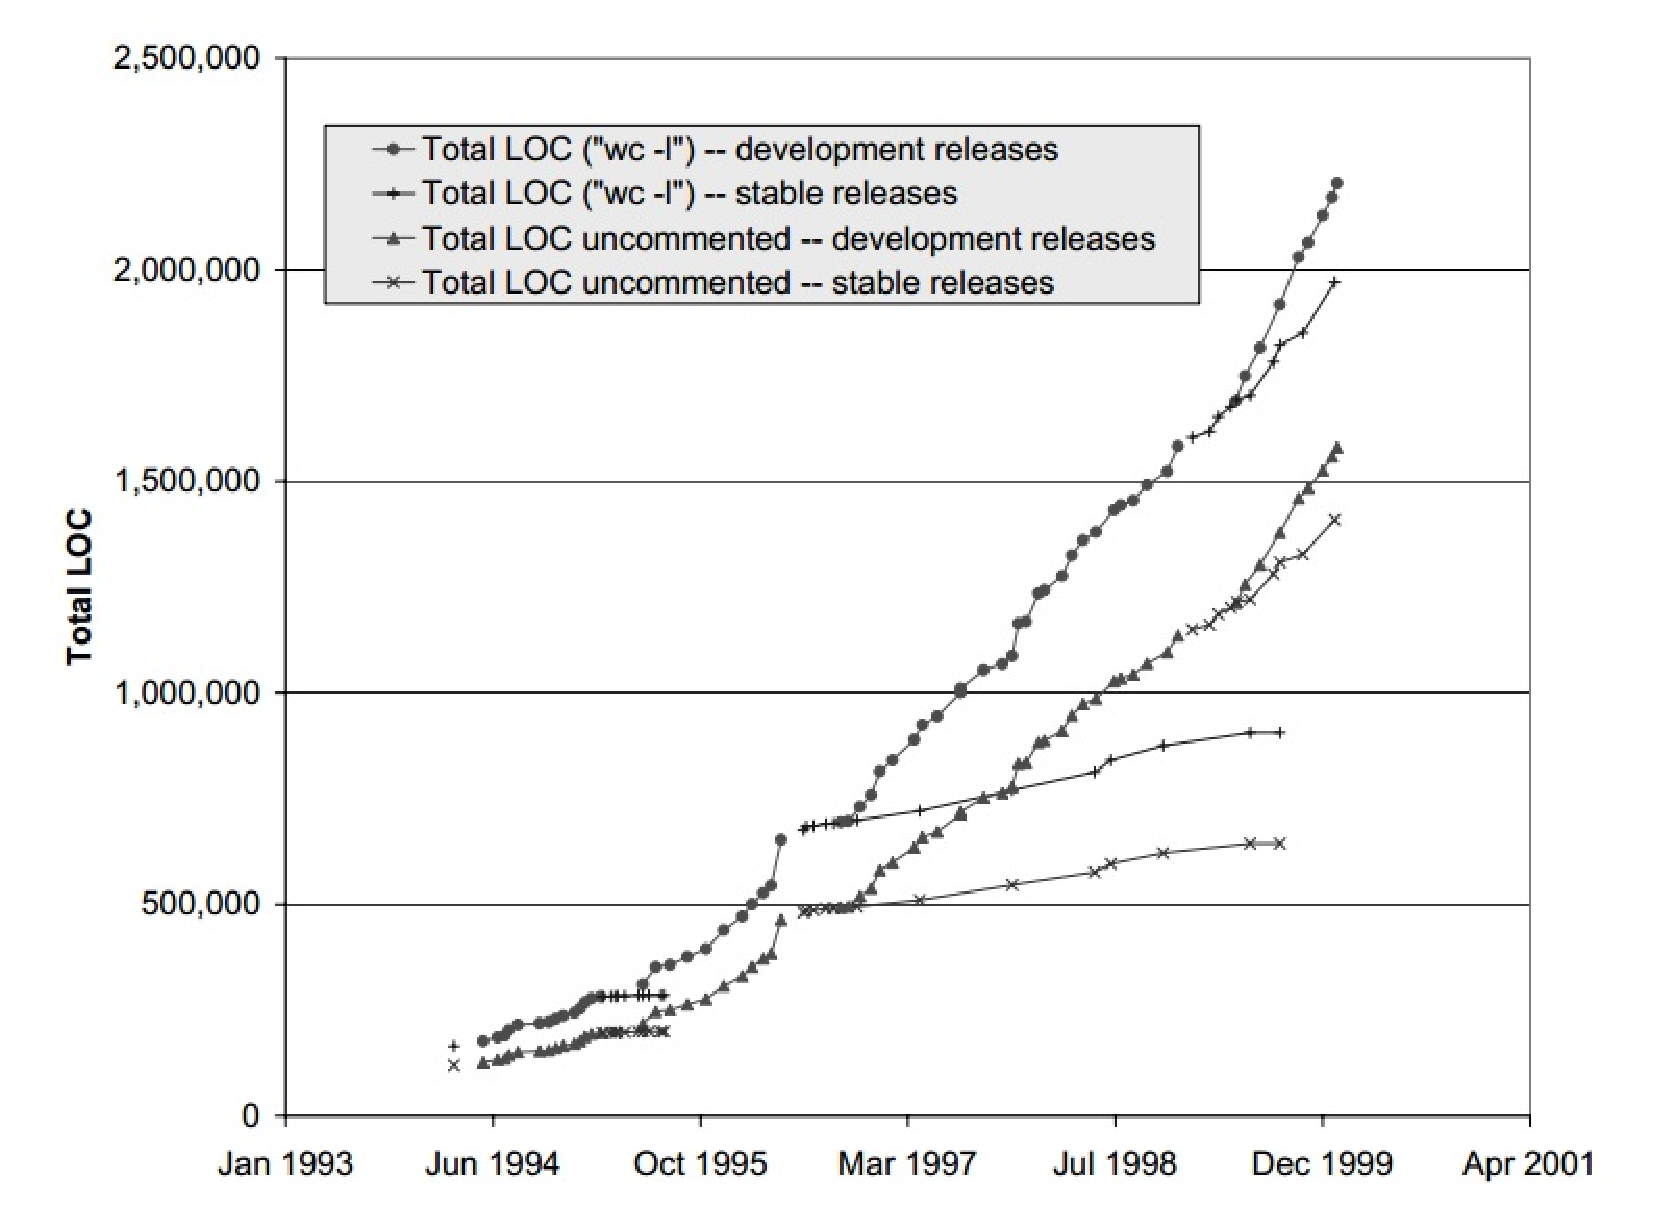
\includegraphics[width=0.6\textwidth]{linux-evolution}
\caption{Evolução do sistema operacional Linux, extraído de \cite{godfrey2000evolution}}
\label{fig-evolucaolinux}
\end{figure}

Os dados presentes no gráfico, até o início dos anos 2000, vão de encontro à quinta lei de Lehman, citada na Tabela \ref{tab-leis-lehman}. No gráfico, o número de linhas de código (LOC) do kernel do sistema, possui taxa de crescimento positiva, enquanto a lei afirma que ao longo do tempo a taxa de crescimento tende a diminuir.
%
Por outro lado, neste trabalho, não estamos tratando a evolução de software do ponto de vista da inserção de novas funcionalidades, o que pode levar ao crescrimento de número de linhas de código, como exemplificado acima. Estamos tratando a evolução de um software livre real, do ponto de vista da sua arquitetura, de acordo com as decisões julgadas pelo seus principais desenvolvedores, conforme descrito nas respostas ao questionário apresentado no Apêndice \ref{form-pesquisa}, para poderem evoluir o projeto de uma forma mais rápida e objetivando formação de uma comunidade de desenvolvedores.

\section{Visualização de Informação em Softwares Livres}

%Contexto e conceito e importência da visualização

O desenvolvimento de softwares livres pode ser referenciado como um movimento que vem sendo pesquisado e aplicado em grandes organizações, assim como vem sendo utilizados por um grande número de desenvolvedores em todo mundo. Apesar disso é um movimento recente, o que causa certa resistência na adoção dessa nova abordagem por um número maior de organizações e desenvolvedores. Isso pois inicialmente havia certa dificuldade na seleção e integração desses produtos, o que motivou o estabelecimento de processos objetivos para compreensão da qualidade de projetos FOSS. Uma das formas para compreender, é a extração de métricas de qualidade, tanto de código-fonte como de repositório. 

O processo de extração de métricas, muitas vezes, geram um grande volume de informações que são difíceis de análisar em ferramenta apropriada. O objetivo da visualização de informação aplicada a softwares livres é possibilitar que grandes quantidades de informações, as métricas extraídas, sejam analisadas objetivamente para compreensão da qualidade de projetos FOSS. Isso permite estabelecer um processo para apoiar as tarefas de avaliação, monitoramento e melhoria da qualidade.

%Motivação
Muitas vezes sa avaliações de projetos FOSS são feitas informalmente, com a leitura de documentação e análise de opiniões de usuários anteriores, que nem sempre geram resultados confiáveis. Nesses projetos, muitos dados, tanto de processo como de produto, estão disponíveis publicamente. Exemplos desses dados são: código-fonte, históricos de evolução do repositório, conjunto de testes, relatório de erros, entre outros. Todas essas informações, se corretamente processadas, podem ser utilizadas para avaliar a qualidade de projetos. 

Métricas podem ser usadas para medir características e atributos definidos por modelos de qualidade de software voltados para a an análise tanto do processo quanto do produto. Alguns modelos propostos especificamente para FOSS (Deprez e Alexandre, 2008; Petrinja et al., 2009; Spinellis et al., 2009) se baseiam em modelos tradicionais como o CMMI (Capability Maturity Model Integration) (Chrissis et al., 2006) e a norma ISO 9126 (ISO/IEC, 2001) mas incluem extensões que consideram especificamente aspectos importantes do desenvolvimento aberto. No entanto, a multiplicidade de indicadores de qualidade que podem ser extraídos de um projeto FOSS, considerando todas as suas diversas perspectivas (principalmente código, testes e repositório), cada um com sua própria interpretaçãoe valores de referência, torna complicada a realização de uma avaliação objetiva e direta. Abaixo se encontram as métricas disponibilizadas pelas ferramentas base utilizadas na plataforma Mezuro.

\graphicspath{{figuras/}}
\begin{figure}[H]
\centering
\includegraphics[width=0.4\textwidth]{analizo_temp}
\caption{Métricas fornecidas pela ferramenta base Analizo}
\label{fig-evolucaolinu}
\end{figure}

\graphicspath{{figuras/}}
\begin{figure}[H]
\centering
\includegraphics[width=0.4\textwidth]{checkstyle_temp}
\caption{Métricas fornecidas pela ferramenta base Checkstyle}
\label{fig-evolucaolin}
\end{figure}

Plataformas de avaliação de qualidade baseadas em conjuntos de ferramentas, como é o caso da plataforma Mezuro, expõem o avaliador de qualidade a dezenas de valores numéricos relacionados as métricas calculadas. Sem uma apresentação especial, esses dados são de pouco valor, pois são numerosos e difíceis de avaliar. Muitas vezes as métricas não são correlacionadas e a formatação da apresentação consiste apenas na aplicação de valores de referência.

Uma possibilidade para a solução desse problema é o uso de visualização de informação, que são representações visuais e interativas de dados, apoiadas por computador, utilizadas para amplificar a aquisição de conhecimento e apoiar descobertas, tomadas de decisão e explicações a partir de dados complexos.

Uma das ramificações da visualização de informação que mais cresce atualmente á a visualização de software, cujos objetivos são auxiliar a compreensão de sistemas complexos de software e melhorar a produtividade do processo de desenvolvimento utilizando visualização. A visualização de software é dividida em três categorias principais: estrutura, comportamento e evolução.

%tecnicas para visualização em geral: https://github.com/mbostock/d3/wiki/Gallery

\begin{itemize}
\item \textbf{Estrutura} é a categoria que representa as partes estáticas do sistema, ou seja, aquelas que podem ser computadas sem executá-lo. 

%tecnicas de visualição dessa categoria, de acordo com Rafael Messias:
%codecity, treemap, HEB
%Grande parte das ferramentas propostas na categoria Estrutura compartilham um
%mesmo modelo conceitual: a geração de um grafo, onde vértices representam entidades
%do programa, como arquivos ou classes, e arestas representam dependências como usos ou
%heranças. A técnica Hierarchical Edge Bundles (HEB) (Holten, 2006), ilustrada na Figura
%3.3,  ́e utilizada para visualizar ao mesmo tempo duas informações do grafo: a estrutura
%hierárquica dos arquivos do código fonte e suas dependências, ou seja, as chamadas entre
%funções ou métodos.

\item \textbf{Comportamento} se refere a compreensão do que ocorre com o sistema durante seu tempo de execução. Para o Mezuro essa categoria não é tão interessante, já que as métricas analisadas nessa plataforma, são extraídas a partir de sua análise estática.

%As técnicas dessa categoria NÃO são importantes para o Mezuro (pelo menos até agora)

\item \textbf{Evolução} representa as características modificadas ao longo do tempo em um sistema. Técnicas de visualizações dessa categoria podem auxiliar analistas verificarem quais as relações entre artefatos modificados, quais tendências dessas modificações. Analisar e evolução de um sistema pode ser tão ou mais importante que a análise de sua estrutura, já que manutenções, sejam elas corretivas, preventivas ou adaptatiavs representam grande parte do custo envolvido em um projeto, podendo chegar em até 80\% do total.

%técnicas presentes na categoria de evolução:
%
%
%

\end{itemize}













